\FloatBarrier
\section{Causal Estimation}

A data-generating process that has survived Stage 3 licenses the full estimation pipeline, conditional on the ignorability assumption that Section 3.4 identifies. This section carries out the intervention rung of Pearl's ladder of causation on the Chicago data.

\subsection{The Experimental Question and the Two Analysts}

To demonstrate causal knowledge's contribution to the analytical process, we consider a theoretical situation: two analysts face the same dataset, the same research question, and the same methods, differing only in whether they are aware of the tested DGP. Both pursue the same objective, a model of emissions valid for the entire building stock, and any difference in their analyses is then attributable to causal knowledge alone.

Awareness of the tested DGP does not alter the causal analyst's objective; it alters the interpretation of the data at hand. The sample represents $P(Y \mid X, C = 1)$; the analyst recognises this as a biased view of the population $P(Y \mid X)$. The bias is corrected by reweighting the sample toward the population, the back-door adjustment the gate requires (Section 3.4). The tested DGP also determines the predictor set: the upstream causes alone, $\mathbf{X}_s$, $X_o$, and the period index. Mediators and derived fields are withheld as downstream of those causes. Cross-validation is grouped by building, so that no building appears in both the training and test folds. The resulting model targets the population relationship $P(Y \mid X)$, corrected for the selection the gate induces.

Unaware of the tested DGP, the causally-blind analyst pursues the same objective but interprets the same data differently. The conditional $P(Y \mid X, C = 1)$ is taken to be the population relationship $P(Y \mid X)$, and the reporting subset is treated as representative of the full stock. With no discrepancy perceived, no correction is applied; the task reduces to predicting the recorded emissions as accurately as possible. Every available field is retained as a predictor, the mediators and derived fields among them. The sample is left unweighted, and cross-validation is performed without grouping, ignoring the panel structure. The resulting model fits the reporting buildings well, but is biased as an estimate of the city-wide relationship.

The next section makes the comparison precise, crossing each analyst's pipeline with a range of functional forms.

\subsection{The Factorial Design}

The comparison is made precise by crossing the two pipelines with three functional forms, producing a 2$\times$3 factorial in which each contribution can be isolated independently. The three forms span the two-cultures question (\cit{breiman2001}{Breiman, 2001}): OLS as the classical structural baseline, XGBoost as the algorithmic culture, and a hierarchical Bayesian model as the structural culture with calibrated uncertainty.

{
\footnotesize
\setlength{\tabcolsep}{5pt}
\renewcommand{\arraystretch}{1.15}
\begin{longtable}{lrr}
\toprule
 & Causally blind & Causal pipeline \\
\midrule
\endfirsthead
\toprule
 & Causally blind & Causal pipeline \\
\midrule
\endhead
\bottomrule
\endlastfoot
\textbf{Linear} & M1: CB OLS & M4: IPW OLS \\
\textbf{Flexible (algorithmic)} & M2: CB XGBoost & M5: IPW XGBoost \\
\textbf{Flexible (structural)} & M3: CB Hierarchical Bayes & M6: IPW Hierarchical Bayes \\
\end{longtable}
}

The factorial structure separates the two contributions by holding one fixed while varying the other. Reading down a column holds the functional form fixed and varies only the pipeline, so any performance difference is attributable to the causal correction alone. Reading across a row holds the pipeline fixed and varies only the functional form. The comparison of primary interest is M5 against M6: both target the same population quantity from the same upstream features, and agreement between them on MdAPE is evidence that the tested DGP is sufficient to identify the population relationship (Section 3.4).

Four design choices separate the two pipelines, each determined by the tested DGP rather than by convention.

\begin{enumerate}
  \item \textbf{Feature set.} The causal pipeline uses the upstream causes only: $\mathbf{X}_s$, $X_o$, and the period index. The causally-blind pipeline retains every available field, including the mediators and derived performance fields.
  \item \textbf{Row subset.} The causal pipeline trains on compliant records only. The causally-blind pipeline trains on all records with an observed target, a slightly larger sample that nonetheless describes only the reporting buildings. This asymmetry is deliberate: each pipeline receives the data exactly as its analyst would actually prepare it.
  \item \textbf{Selection correction.} The causal pipeline reweights observations by the inverse propensity of compliance. The causally-blind pipeline applies no reweighting.
  \item \textbf{Cross-validation protocol.} The causal pipeline groups all observations of a building into the same fold (GroupKFold on building identity), reflecting the panel structure. The causally-blind pipeline uses ordinary $k$-fold, treating each row as independent.
\end{enumerate}

\subsection{The Propensity Model}

Selection is corrected by estimating the probability of compliance as a function of the upstream features. A logistic regression of the compliance indicator $C$ on $\mathbf{X}_s$, $X_o$, and the period index yields propensity scores $\hat{e}(X) = P(C = 1 \mid X)$. Property type is one-hot encoded because the ordinance defines the reporting obligation categorically by property class, with no ordinal structure across the 63 types the dataset records (Sections 4.1, 4.4). The period index is included because the tested DGP marks it as a parent of the compliance gate (Figure 4.8); the ordinance was phased in over successive years, so the probability of compliance depends on timing as well as building characteristics.

The model is fitted on all 28,329 records, compliant and non-compliant alike, since the gate can be learned only from both sides. This requires the upstream features to be complete, and in the raw file they are not: floor area is null in 7.8\% of records, property type in 15.0\%, year built in 17.8\%, and building count in 15.7\% (Section 4.1). A single shared preprocessing step, applied before either pipeline runs, fills the numeric upstream features with their global medians computed over all 28,329 records prior to any filtering, and assigns missing property types an explicit Unknown category that is one-hot encoded like any other class. This is the preprocessing step that the class definition of Section 2.1 anticipates for upstream fields with real missingness; it is identical for the causal and causally-blind pipelines, so no difference between their results can originate in it. Inputs are standardised before the logistic fit.

The resulting weights are moderate, indicating adequate overlap on the observed upstream characteristics. Raw inverse probability weights $w_i = 1 / \hat{e}(X_i)$ are trimmed at the 99th percentile and normalised to mean one (\cit{colehernan2008}{Cole \& Hernán, 2008}); the largest resulting weight is 1.32, so even the most underrepresented compliant building exerts only 32\% more influence than average. The propensity model classifies compliance at 95.1\% accuracy on the full dataset. The correction addresses selection on observed covariates only; selection on unobserved factors such as building management quality or retrofit investment is not corrected and is carried as a limitation.

The back-door correction is applied in both model families through mechanisms suited to each. In the OLS and XGBoost models, the weights enter as observation weights in the fitting procedure. In the hierarchical Bayesian models, they are injected via a likelihood potential,

\[
\log p^*(\theta \mid \text{data}) = \log p(\theta \mid \text{data}) + \sum_i (w_i - 1) \cdot \log p(y_i \mid \mu_i, \sigma),
\]

which up-weights the log-likelihood contribution of underrepresented buildings in proportion to their normalised weight. This is the back-door adjustment of Section 3.4, applied at the level of the posterior (\cit{pearl2009}{Pearl, 2009, Ch. 3}).

\subsection{Model Specifications}

\textbf{OLS (M1 and M4).} Both models assume a linear relationship between the feature vector and the log-transformed outcome. For observation $i$, the model is:

\[
y_i \sim \text{Normal}(\mu_i,\; \sigma), \qquad \mu_i = \mathbf{x}_i^\top \boldsymbol{\beta}
\]

where $y_i = \log_{1+}(\text{GHG}_i)$, $\mathbf{x}_i$ is the feature vector including an intercept, and $\boldsymbol{\beta}$ is the coefficient vector. Minimising the residual sum of squares yields the closed-form OLS estimator:

\[
\hat{\boldsymbol{\beta}} = (\mathbf{X}^\top \mathbf{X})^{-1} \mathbf{X}^\top \mathbf{y}
\]

where $\mathbf{X}$ is the $n \times p$ design matrix and $\mathbf{y}$ is the $n$-vector of log-transformed outcomes. No hyperparameters are tuned.

M1 and M4 differ in feature set, row subset, and whether IPW reweighting is applied. M1 trains on the full causally-blind feature set ($N = 21{,}714$ rows) with no reweighting; string and boolean columns (property type, ZIP code, community area, reporting status, exempt flag) are one-hot encoded. M4 trains on upstream features only ($N = 21{,}406$ compliant rows), with property type one-hot encoded, and replaces the OLS estimator with its IPW-weighted counterpart:

\[
\hat{\boldsymbol{\beta}}_{\text{WLS}} = (\mathbf{X}^\top \mathbf{W} \mathbf{X})^{-1} \mathbf{X}^\top \mathbf{W} \mathbf{y}
\]

where $\mathbf{W} = \mathrm{diag}(w_1, \ldots, w_n)$ and $w_i$ is the normalised IPW weight for observation $i$ derived from the propensity model (Section 5.3).

\textbf{XGBoost (M2 and M5).} Both XGBoost models approximate the conditional expectation $\mathbb{E}[\log_{1+}(\text{GHG}) \mid \mathbf{x}]$ as an additive ensemble of $T$ regression trees (Chen \& Guestrin, 2016), a flexible nonparametric form that imposes no assumed functional relationship between GHG emissions and the input features:

\[
\hat{y}_i = \sum_{t=1}^{T} f_t(\mathbf{x}_i), \quad f_t \in \mathcal{F}
\]

where $\mathcal{F}$ is the space of regression trees with leaf weight vectors $\mathbf{w}_t$. At each boosting step, a new tree is fitted to the negative gradient of a squared-error loss in $\log_{1+}$ space. Complexity is penalised via

\[
\Omega(f_t) = \gamma L_t + \tfrac{1}{2}\lambda \|\mathbf{w}_t\|^2 + \alpha \|\mathbf{w}_t\|_1
\]

where $L_t$ is the number of leaves, $\gamma$ is the minimum loss reduction required to admit a split, $\lambda$ is L2 regularisation on leaf weights, and $\alpha$ is L1 regularisation. Additional capacity is controlled by the maximum tree depth, subsampling ratio (fraction of training observations drawn per tree), column-sampling ratios at the tree and node levels, and the minimum child weight (minimum total instance weight in a child node).

Both models are tuned via nested cross-validation, which keeps the hyperparameter search separate from the generalisation estimate so that the reported CV performance reflects a model tuned on the training data alone. The outer loop provides five independent evaluation folds; within each, an Optuna Tree-structured Parzen Estimator (TPE; Akiba et al., 2019) runs 60 trials on a three-fold inner loop, searching jointly over all capacity and regularisation hyperparameters listed above. The inner loop uses MdAPE as the Optuna objective, so hyperparameter selection directly optimises the primary evaluation metric; within each trial, XGBoost early stopping uses RMSE with a 30-round patience. The winning configuration is applied to the full outer-fold training set with $n_{\text{estimators}} = 2{,}000$ and a 50-round early-stopping patience; $n_{\text{jobs}} = 1$ ensures deterministic floating-point accumulation. The deployment model refits on all available training data under the hyperparameter configuration from the median inner tuning run. Categorical columns are label-encoded and boolean columns are coerced to integer; numeric columns are filled with their within-fold median.

M2 and M5 are architecturally identical but differ in the four pipeline respects established in Section 5.2. M2 trains on the full causally-blind feature set ($N = 21{,}714$ rows) under \code{KFold} with no IPW correction. M5 trains on upstream features only ($N = 21{,}406$ compliant rows) under \code{GroupKFold} on building identity, and IPW enters as sample weights passed to the XGBoost \code{fit} call. The \code{GroupKFold} structure is maintained in both the inner tuning loop and the outer evaluation folds, so that no building appears in both training and test sets at any stage of the M5 pipeline.

\textbf{M3, Causally-Blind Hierarchical Bayes.} M3 is a hierarchical Normal regression in $\log_{1+}$(GHG) space over upstream features and five fuel-type mediators, trained on the full causally-blind row set ($N = 21{,}714$) with no IPW correction. The full generative model is:

\[
\begin{aligned}
y_i &\sim \text{Normal}(\mu_i,\; \sigma) \\
\mu_i &= \alpha_{j[i]} + \beta_A \tilde{a}_i + \beta_B \tilde{b}_i + \beta_T \tilde{t}_i + \beta_Y \tilde{y}_i \\
      &\phantom{{}={}}\quad + \beta_E \tilde{e}_i + \beta_G \tilde{g}_i + \beta_S \tilde{s}_i + \beta_W \tilde{w}_i + \beta_O \tilde{o}_i \\
\alpha_j &= \bar{\alpha} + \delta_j \sigma_\alpha \\
\delta_j &\sim \text{Normal}(0,\; 1), \quad j = 1, \ldots, 63 \\
\bar{\alpha} &\sim \text{Normal}(7.0,\; 1.0) \\
\sigma_\alpha &\sim \text{HalfNormal}(1.0) \\
\beta_k &\sim \text{Normal}(0,\; 2.5), \quad k \in \{A, B, T, Y\} \\
\beta_f &\sim \text{Normal}(0,\; 2.0), \quad f \in \{E, G, S, W, O\} \\
\sigma &\sim \text{HalfNormal}(0.5)
\end{aligned}
\]

where $\tilde{a}_i$ and $\tilde{b}_i$ are log floor area and log building count centred at their training-fold means; $\tilde{t}_i$, $\tilde{y}_i$, $\tilde{e}_i$, $\tilde{g}_i$, $\tilde{s}_i$, $\tilde{w}_i$, $\tilde{o}_i$ are data year, year built, electricity, natural gas, district steam, district chilled water, and other fuel use, each standardised to zero mean and unit variance within the training fold. The global intercept prior $\text{Normal}(7.0, 1.0)$ is centred at $\exp(7) \approx 1{,}097$ metric tons CO$_2$e, close to the observed stock median, placing a weakly informative anchor on the unconditional GHG level. The upstream slope priors $\text{Normal}(0, 2.5)$ are agnostic about log-scale elasticities, reflecting the blind analyst's absence of structural prior knowledge about how area, age, or building count relate to emissions. The mediator priors $\text{Normal}(0, 2.0)$ are wide enough to allow the fuel slopes to recover the EPA emission-factor magnitudes from the data without constraining their values, while remaining informative enough to exclude implausibly large slopes. The non-centred parameterisation $\alpha_j = \bar{\alpha} + \delta_j \sigma_\alpha$ is required for NUTS convergence under weakly identified hierarchical parameters. The derived metrics, spatial indices, and compliance metadata present in the causally-blind training set are excluded from the likelihood. M3's generative model assigns explicit slope parameters only to upstream features and fuel mediators; those additional columns are available in the training data but do not enter the likelihood. The hierarchy spans all 63 property types in the causally-blind dataset. Like M6, M3 is evaluated via PSIS-LOO rather than held-out folds.

\textbf{M6, Causal Hierarchical Bayes.} M6 is a hierarchical Normal regression in $\log_{1+}$(GHG) space, fitted to the compliant row set ($N = 21{,}406$) with IPW applied via a likelihood potential. The full generative model is:

\[
\begin{aligned}
y_i &\sim \text{Normal}(\mu_i,\; \sigma) \\
\mu_i &= \alpha_{j[i]} + \beta_A \tilde{a}_i + \beta_B \tilde{b}_i + \beta_T \tilde{t}_i + \beta_Y \tilde{y}_i \\
\alpha_j &= \bar{\alpha} + \delta_j \sigma_\alpha \\
\delta_j &\sim \text{Normal}(0,\; 1), \quad j = 1, \ldots, 55 \\
\bar{\alpha} &\sim \text{Normal}(7.0,\; 1.0) \\
\sigma_\alpha &\sim \text{HalfNormal}(1.0) \\
\beta_k &\sim \text{Normal}(0,\; 0.5), \quad k \in \{A, B, T, Y\} \\
\sigma &\sim \text{HalfNormal}(0.5)
\end{aligned}
\]

where $\tilde{a}_i$ and $\tilde{b}_i$ are log floor area and log building count centred at their training-fold means, and $\tilde{t}_i$ and $\tilde{y}_i$ are data year and year built standardised to zero mean and unit variance. The global intercept prior $\text{Normal}(7.0, 1.0)$ is centred at $\exp(7) \approx 1{,}097$ metric tons CO$_2$e, close to the observed compliant-stock median. The non-centred parameterisation is required for NUTS convergence under weakly identified hierarchical parameters, as in M3. The upstream slope priors $\text{Normal}(0, 0.5)$ encode the causal analyst's expectation of near-unit log-scale elasticities: Stage 3 estimated the log-floor-area elasticity at approximately 1.0, meaning doubling floor area roughly doubles GHG emissions. This prior places 95\% of mass within $[-1, 1]$, encoding the expectation without constraining the remaining upstream slopes rigidly. IPW is injected via a likelihood potential (Section 5.3); the hierarchy spans the 55 property types present in the compliant training set.

Both Bayesian models share the same priors on $\sigma_\alpha$ and $\sigma$. The prior $\text{HalfNormal}(1.0)$ on $\sigma_\alpha$ allows type-level intercepts to vary by approximately $\pm 1$ log unit around the global mean, equivalent to a factor of $e \approx 2.7$ between the most and least emissions-intensive property types; this is consistent with the heterogeneity observed across office, warehouse, and multifamily residential building classes. The prior $\text{HalfNormal}(0.5)$ on $\sigma$ is weakly informative: a residual standard deviation of 0.5 on the log scale corresponds to multiplicative prediction errors of $\exp(0.5) \approx 1.65$ in the original scale, placing a soft upper bound on unexplained variation while leaving the data to determine the actual residual magnitude.

Both models are sampled with four chains, 3,000 warmup steps, and 3,000 post-warmup draws, using a target acceptance rate of 0.95 and \code{jitter+adapt\_diag} initialisation. Convergence is assessed by $\hat{R} < 1.01$ and bulk effective sample size $> 400$ for all structural parameters (\cit{vehtarietal2021}{Vehtari et al., 2021}). Predictive performance is evaluated via Pareto-smoothed importance-sampling leave-one-out cross-validation (PSIS-LOO; \cit{vehtarietal2017}{Vehtari et al., 2017}).

\subsection{Evaluation Metrics and Ex-Ante Predictions}

Each model is evaluated on five metrics: $R^2(\log)$, MdAPE, median RMSE, 89\% predictive interval coverage, and ELPD. Models are fitted and evaluated in $\log_{1+}$(GHG) space; point metrics ($R^2(\log)$ and RMSE) are reported on this scale. Together the five metrics capture complementary aspects of model performance that no single metric covers simultaneously for a right-skewed outcome: point accuracy, scale-invariant error, interval calibration, and predictive density.

\begin{enumerate}
  \item \textbf{$R^2(\log)$} is the proportion of log-scale variance explained. Values near 1.0 are expected whenever a model has access to near-identity inputs; an unusually high $R^2(\log)$ in this design is a diagnostic signal rather than a performance achievement.
  \item \textbf{MdAPE} is the primary evaluation metric. The median absolute percentage error is scale-invariant and per-building: a value of 20\% means the median building's estimate deviates from its true value by roughly a fifth, a quantity a policy analyst can reason about directly. MdAPE is preferred over mean-based error metrics because GHG emissions are right-skewed; a small number of very large buildings dominate absolute-error averages, making them uninformative for the typical building. Building-level GHG emissions vary substantially even among buildings with similar physical characteristics, due to occupant behaviour, equipment age, and operational schedules, all sources of variation that upstream physical features cannot capture and that set a practical floor on prediction error.
  \item \textbf{Median RMSE} is reported in metric tons CO$_2$e on the original scale. For OLS and XGBoost (M1, M2, M4, M5), RMSE is computed on the held-out test fold at each of the five CV splits and the median is taken across folds. For the Bayesian models (M3 and M6), there are no KFold splits; RMSE is instead computed from PSIS-LOO leave-one-out predictive means against observed values. The two procedures are on different computational bases and Bayesian RMSE values should not be compared directly to frequentist fold-median values.
  \item \textbf{89\% predictive interval coverage} reports the fraction of held-out observations that fall inside the model's 89\% predictive band. Values above 89\% indicate conservatively wide intervals; values below indicate over-confident intervals.
  \item \textbf{ELPD} is the primary criterion for the Bayesian models (M3 and M6). PSIS-LOO ELPD is a sum of log predictive densities; higher values indicate better-calibrated predictive distributions, and differences larger than roughly four units are practically meaningful. Because ELPD accumulates over observations, raw values are not directly comparable between models fitted on different row subsets. For OLS and XGBoost, ELPD is estimated via a normal approximation applied to CV prediction errors, since these models do not produce posterior predictive distributions; for the Bayesian models, ELPD is computed exactly via PSIS-LOO from the full posterior. The two methods are directionally consistent but not strictly on the same computational basis.
\end{enumerate}

The four predictions below follow from the experimental structure and the tested DGP alone; none draws on the results that Section 5.6 reports, so their corroboration or refutation is informative about the DGP's implications rather than fitted to the outcomes after the fact.

\begin{enumerate}
  \item \textbf{Convergence.} On the corrected foundation, M5 (IPW XGBoost) and M6 (IPW Hierarchical Bayes) will agree on MdAPE to within roughly one percentage point. With the tested DGP specifying the causal structure, the structural and algorithmic estimators answer the same population-level question and have no quantity to disagree about.
  \item \textbf{The cost of correction.} Within every functional form, the causal pipeline will show higher apparent cross-validation error than its causally-blind counterpart. The blind advantage reflects selection and co-outcome leakage, not generalisation; its presence is expected and informative rather than a failure of the causal pipeline.
  \item \textbf{The accounting artefact.} The causally-blind XGBoost (M2) will attain unusually low cross-validation error by exploiting derived fields (site EUI, source EUI, national median EUI) that encode a near-identity with the GHG outcome. SHAP mediator attribution will confirm that this apparent accuracy reflects an accounting relationship rather than predictive skill over upstream inputs.
  \item \textbf{Deployment separation.} Applied to non-compliant buildings, the causal models will produce stable and well-defined estimates; the causally-blind models will produce unreliable estimates, because their derived-field predictors are unobserved for buildings that never reported.
\end{enumerate}

\subsection{Results and Diagnostics}

\subsubsection*{Experimental Results}

Table 5.1 below reports out-of-sample $R^2(\log)$, MdAPE, median RMSE, 89\% predictive interval coverage, and ELPD for all six models; Figure 5.1 plots the same results for visual comparison. The bottom panel of Table 5.1 reports the IPW effect as the difference between causal and causally-blind within each functional form; a positive value indicates the causal pipeline has higher apparent error. Results are discussed in the order of the four ex-ante predictions from Section 5.5.

\par\medskip\noindent
{\small\itshape \textbf{Table 5.1. Out-of-sample results, 2$\times$3 factorial experiment.} The bottom panel (IPW effect = causal minus causally-blind) shows that the causal pipeline records higher apparent CV error for OLS (+8.0 pp) and ML (+18.9 pp); this is expected, as the causally-blind advantage reflects circular feature leakage rather than genuine predictive skill. The convergence of M5 and M6 to within 0.4 pp is the central finding: XGBoost and Hierarchical Bayes agree because the tested DGP fixes the target quantity. The near-zero M3--M6 Bayesian gap and its deployment implications are examined in the diagnostics below. †Bayesian RMSE and ELPD use different computational bases from frequentist models; see Section 5.5 for details.\par}
\nopagebreak\medskip\nopagebreak
{
\footnotesize
\setlength{\tabcolsep}{5pt}
\renewcommand{\arraystretch}{1.15}
\begin{longtable}{lrrrrrr}
\toprule
Pipeline & Model & $R^2(\log)$ & MdAPE & Med. RMSE† & 89\% PI cov. & ELPD \\
\midrule
\endfirsthead
\toprule
Pipeline & Model & $R^2(\log)$ & MdAPE & Med. RMSE† & 89\% PI cov. & ELPD \\
\midrule
\endhead
\bottomrule
\endlastfoot
\textbf{Causally-blind} & M1 OLS & +0.756 & 31.5\% & 174,020 & 93.8\% & -17,075 \\
 & M2 XGBoost & +0.993 & 2.1\% & 1,185 & 96.7\% & +22,317 \\
 & M3 Hier. Bayes† & +0.848 & 20.9\% & 213 & 92.4\% & -11,935 \\
\textbf{Causal} & M4 OLS & +0.557 & 39.5\% & 129,691 & 93.1\% & -22,716 \\
 & M5 XGBoost & +0.835 & 21.0\% & 2,584 & 92.4\% & -12,491 \\
 & M6 Hier. Bayes† & +0.838 & 21.4\% & 218 & 92.8\% & -12,316 \\
\textbf{IPW effect} (causal - CB) & Frequentist & -0.199 & +8.0 pp & -44,328 & -0.7 pp & -5,641 \\
 & ML & -0.158 & +18.9 pp & +1,399 & -4.3 pp & -34,809 \\
 & Bayesian & -0.010 & +0.4 pp & +5 & +0.4 pp & -378 \\
\end{longtable}
}
\par\medskip

One feature of Table 5.1 needs comment before the predictions are assessed. The six-figure median RMSE values for the two OLS models (M1: 174,020; M4: 129,691 t CO$_2$e) reflect exponential back-transformation rather than a broken pipeline: all models are fitted in $\log_{1+}$ space, and an OLS log-scale error of a few units on one of the largest buildings becomes an original-scale residual of hundreds of thousands of tons, which a squared-error metric then amplifies. MdAPE is the primary metric for precisely this reason (Section 5.5), and the same extrapolation behaviour reappears as the heavy right tails of M1 and M4 in the deployment distributions (Figure 5.2).

\begin{figure}[tbp]
\centering
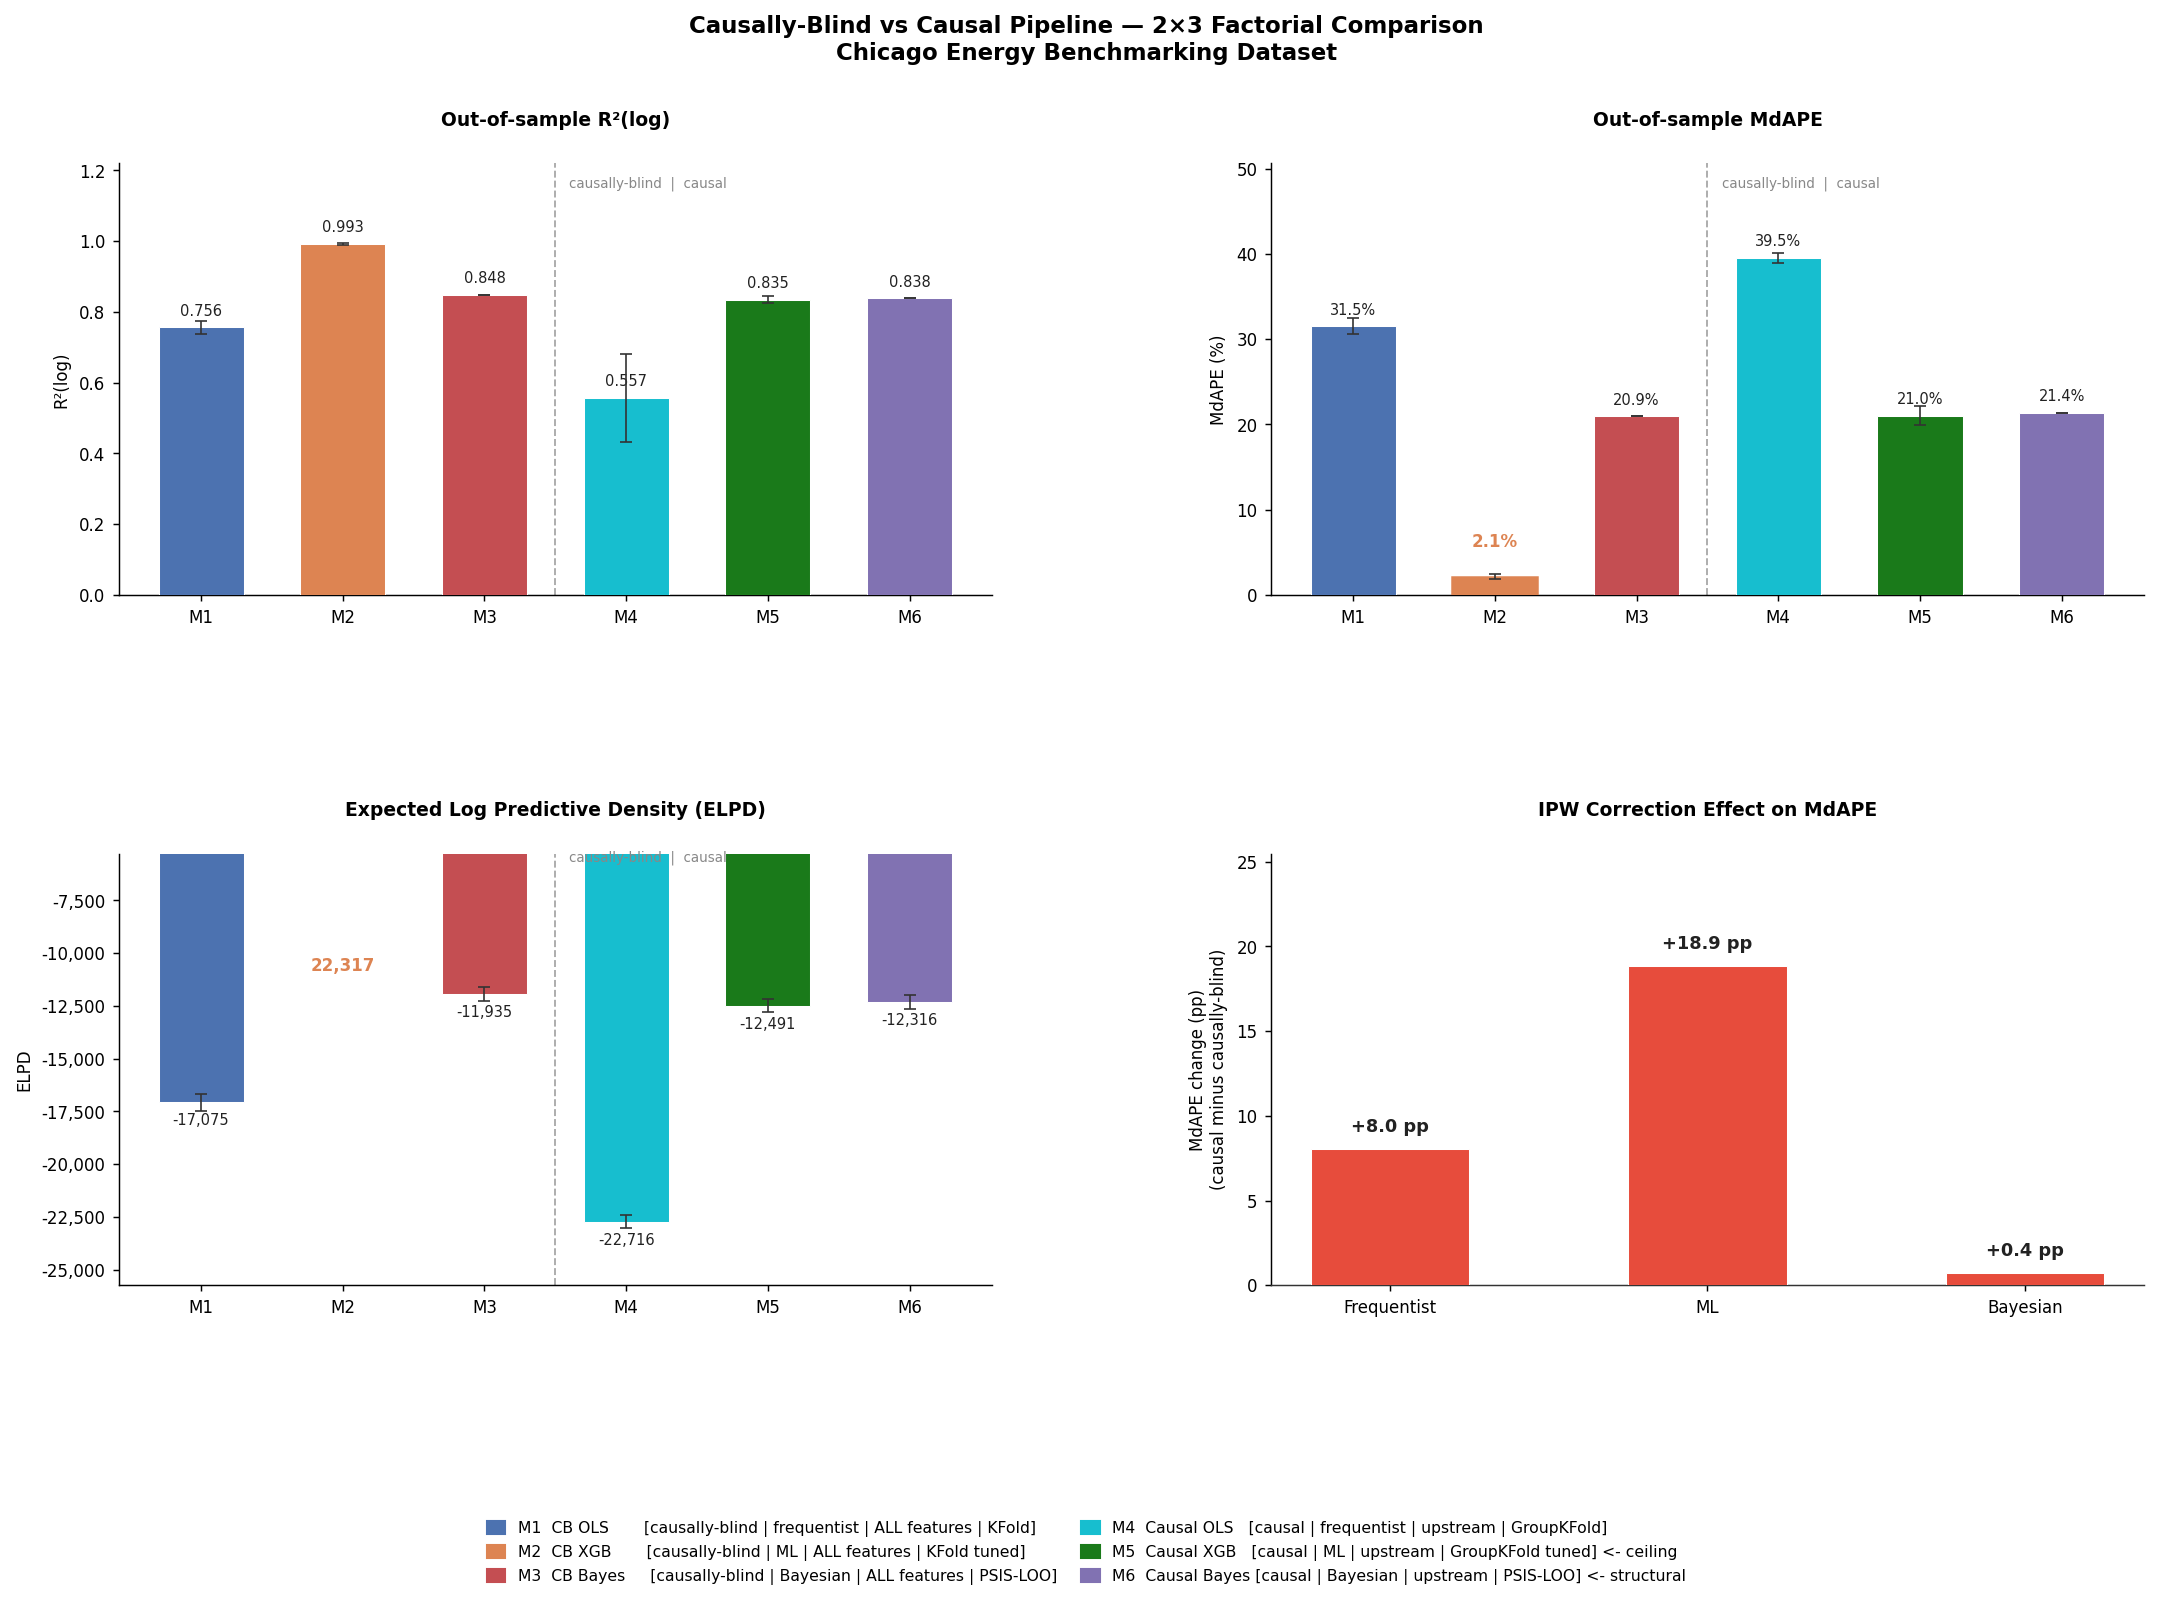
\includegraphics[width=0.95\linewidth]{figures/fig_comparison.png}
\caption*{\textbf{Figure 5.1. Causally-blind vs causal pipeline, 2$\times$3 factorial comparison.} M5 and M6 converge to within 0.4 percentage points on MdAPE; M2 (CB XGBoost) is the clear outlier at 2.1\%. The IPW correction cost is large for OLS (+8.0 pp) and ML (+18.9 pp) but negligible for Bayesian (+0.4 pp). Author's analysis of Chicago Energy Benchmarking data.}
\end{figure}

\textbf{Prediction 1: Convergence (corroborated).} M5 (IPW XGBoost) records MdAPE = 21.0\% and M6 (IPW Hierarchical Bayes) records MdAPE = 21.4\%, a gap of 0.4 percentage points well within the predicted threshold of one percentage point. The convergence holds across the building-size distribution: Figure 5.3 breaks MdAPE down by floor-area quintile, and M5 and M6 remain within 1.5 percentage points of each other across all five quintiles, from the smallest buildings (Q1: 22.5\% vs 22.4\%) to the largest (Q5: 18.3\% vs 18.3\%). The ELPD comparison (M6: $-12{,}316$ versus M5: $-12{,}491$, a difference of 175 units) is marginal and in M6's favour. Where the two estimators agree on prediction, the structural model is preferred: M6 additionally provides interpretable posterior coefficients and calibrated uncertainty intervals at no accuracy cost, and those parameters are the subject of Section 6. This convergence is the paper's central empirical finding: when the data-generating process is tested, structural and algorithmic models estimate the same causal quantity and produce equivalent predictions, resolving the two-cultures tension under the specific condition that the DGP is recoverable from institutional documentation.

MCMC diagnostics confirm reliable sampling for both Bayesian models. M3: $\hat{R}_{\max} = 1.004$, $\text{ESS}_{\min} = 548$, zero divergent transitions, and 5 observations with Pareto-$k > 0.7$ across 21,714 data points (indicating observations whose LOO influence is difficult to estimate reliably). M6: $\hat{R}_{\max} = 1.010$, $\text{ESS}_{\min} = 526$, zero divergent transitions, and 1 observation with Pareto-$k > 0.7$ across 21,406 data points. Both satisfy the $\hat{R} < 1.01$ and bulk $\text{ESS} > 400$ thresholds (\cit{vehtarietal2021}{Vehtari et al., 2021}). The marginally elevated $\hat{R}$ in M6 reflects the additional curvature introduced by the IPW potential in the log-posterior and does not indicate convergence failure.

\textbf{Prediction 2: The cost of correction (corroborated).} $\Delta\text{MdAPE} = \text{MdAPE}_{\text{causal}} - \text{MdAPE}_{\text{CB}}$ is positive in all three approach pairs: $+8.0$ pp for OLS (M4 vs M1), $+18.9$ pp for XGBoost (M5 vs M2), and $+0.4$ pp for Bayesian (M6 vs M3). The causal pipeline records higher apparent CV error in every row of the factorial, as predicted. An analyst reading Table 5.1 without causal domain knowledge would select M2 on CV metrics and deploy a causally invalid model.

\textbf{Prediction 3: The accounting artefact (corroborated).} M2 records $R^2 = 0.993$ and MdAPE = 2.1\% across five KFold splits, with fold-level $R^2$ ranging from 0.989 to 0.996. Figure 5.4 makes the artefact visible: M2's predicted vs actual scatter collapses onto the diagonal with near-zero residual variance, a pattern absent from every other model. Figure 5.3 confirms the artefact is not size-specific: M2's MdAPE is uniformly 1.8--2.8\% across all five floor-area quintiles, ruling out any explanation based on the dominance of a particular building class. The ELPD gap between M2 ($+22{,}317$) and M5 ($-12{,}491$) is 34,808 units, the largest pairwise difference in the factorial. Figure 5.5 traces M2's metrics to SHAP-quantified feature exploitation.

\textbf{Prediction 4: Deployment separation (corroborated).} Table 5.2 and Figure 5.2 report predicted GHG for the 5,510 non-compliant building-year records withheld from all model training. The causal models produce deployment medians of 854 (M4), 1,213 (M5), and 1,043 (M6) metric tons CO$_2$e, a 359-ton range attributable to estimator differences and consistent with the observed compliant-building median of $\approx$1,018 metric tons. Figure 5.2 shows the distribution of predicted GHG across all six models: M5 and M6 produce narrow, overlapping peaks centred near 1,000 metric tons, while M1 and M4 show heavy right tails from OLS extrapolation beyond the compliant training support; M1's mean (2,640 metric tons) is more than five times its median (486) as a result. The causally-blind models span 486 (M1) to 1,025 (M3) metric tons, a 539-ton spread among models nominally using the same data.

\par\medskip\noindent
{\small\itshape \textbf{Table 5.2. Deployment test: predicted GHG for 5,510 non-compliant building-year records.} Median is the primary statistic; means are inflated by OLS extrapolation outliers for M1 and M4. The observed compliant-building median is $\approx$1,018 metric tons CO$_2$e. Causal models cluster near this anchor; causally-blind models span a 539-ton range because each estimates a different effective quantity. Author's analysis of Chicago Energy Benchmarking data.\par}
\nopagebreak\medskip\nopagebreak
{
\footnotesize
\setlength{\tabcolsep}{5pt}
\renewcommand{\arraystretch}{1.15}
\begin{longtable}{lrrr}
\toprule
Model & Pipeline & Median (t CO$_2$e) & Mean (t CO$_2$e) \\
\midrule
\endfirsthead
\toprule
Model & Pipeline & Median (t CO$_2$e) & Mean (t CO$_2$e) \\
\midrule
\endhead
\bottomrule
\endlastfoot
M1 CB OLS & Causally-blind & 486 & 2,640 \\
M2 CB XGBoost & Causally-blind & 641 & 968 \\
M3 CB Hier. Bayes & Causally-blind & 1,025 & 1,184 \\
M4 Causal OLS & Causal & 854 & 3,865 \\
M5 Causal XGBoost & Causal & 1,213 & 1,701 \\
M6 Causal Hier. Bayes & Causal & 1,043 & 1,323 \\
\end{longtable}
}
\par\medskip

\begin{figure}[tbp]
\centering
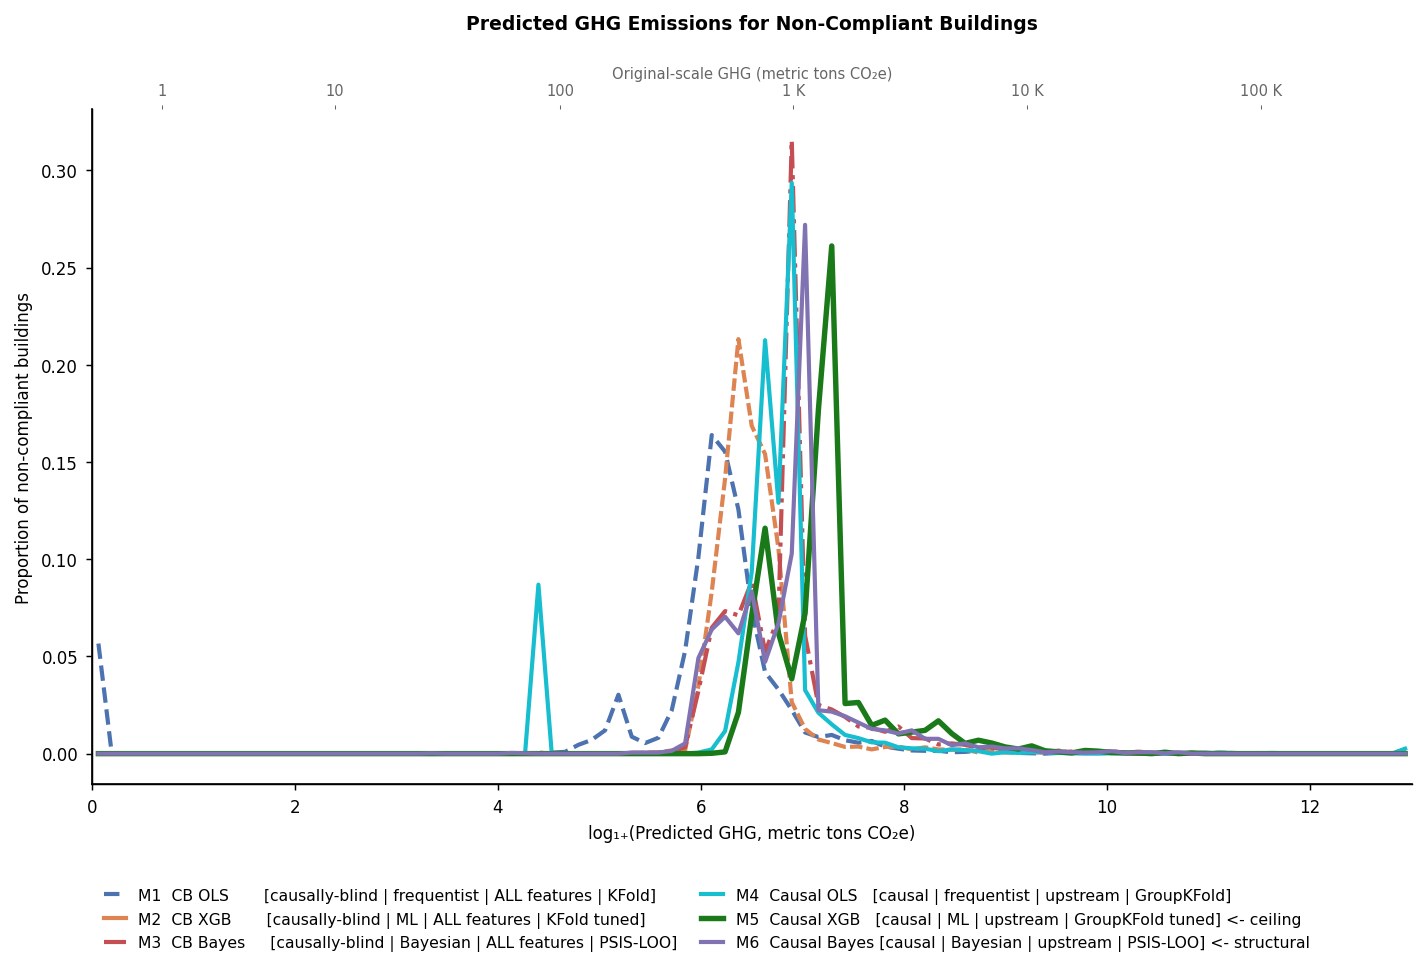
\includegraphics[width=0.95\linewidth]{figures/fig_deployment.png}
\caption*{\textbf{Figure 5.2. Predicted GHG emissions for 5,510 non-compliant building-year records.} Causal models (solid curves) converge on a narrow peak near 1,000 metric tons; causally-blind models (dashed curves) scatter across a 539-ton spread because each exploits the circular features differently and estimates a different effective quantity. M1's heavy right tail and M2's leftward shift are the signatures of OLS extrapolation and near-identity exploitation respectively. Author's analysis of Chicago Energy Benchmarking data.}
\end{figure}

\subsubsection*{Diagnostic Analysis}

The following diagnostics examine the mechanisms behind three results above: M2's near-perfect artefact, the near-zero Bayesian gap, and the divergence of causal and causally-blind models at deployment.

\begin{figure}[tbp]
\centering
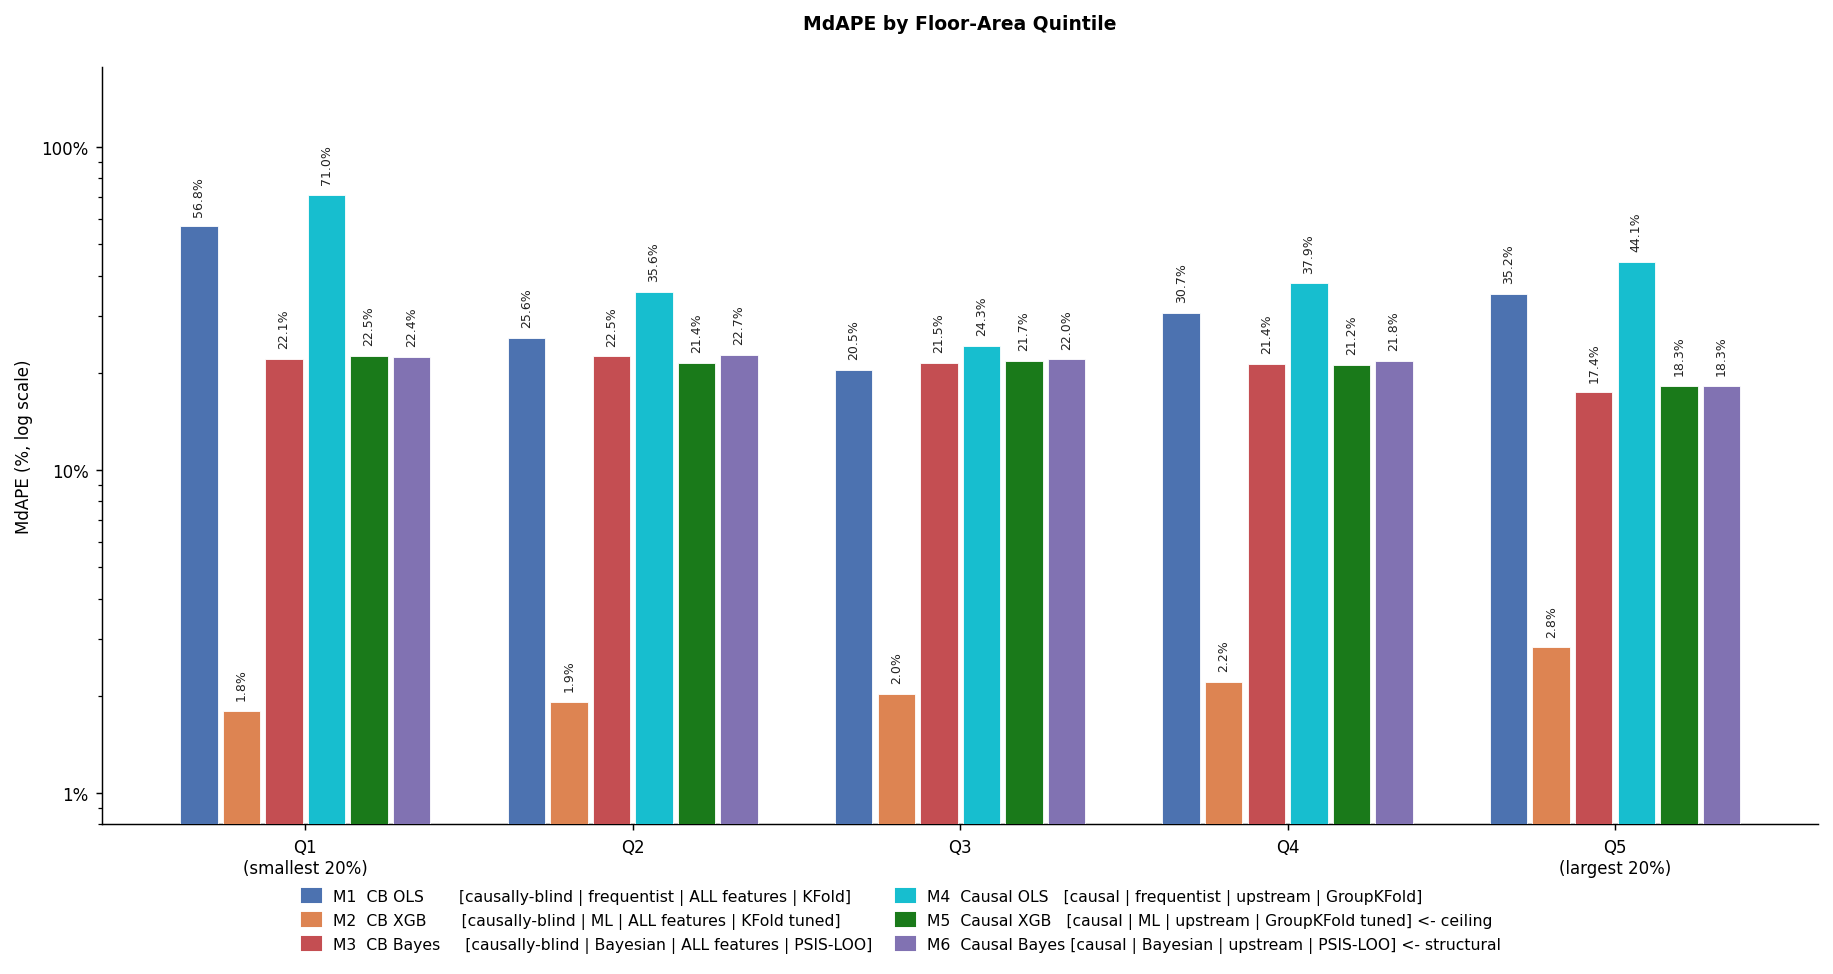
\includegraphics[width=0.95\linewidth]{figures/fig_quintile.png}
\caption*{\textbf{Figure 5.3. MdAPE by floor-area quintile, all six models.} Convergence of M5 and M6 holds at every floor-area quintile, ruling out a size-composition artefact behind the aggregate 0.4 pp gap. M2's MdAPE is uniformly near-zero across all quintiles, confirming the accounting artefact is structural rather than driven by any particular building class. Author's analysis of Chicago Energy Benchmarking data.}
\end{figure}

\begin{figure}[tbp]
\centering
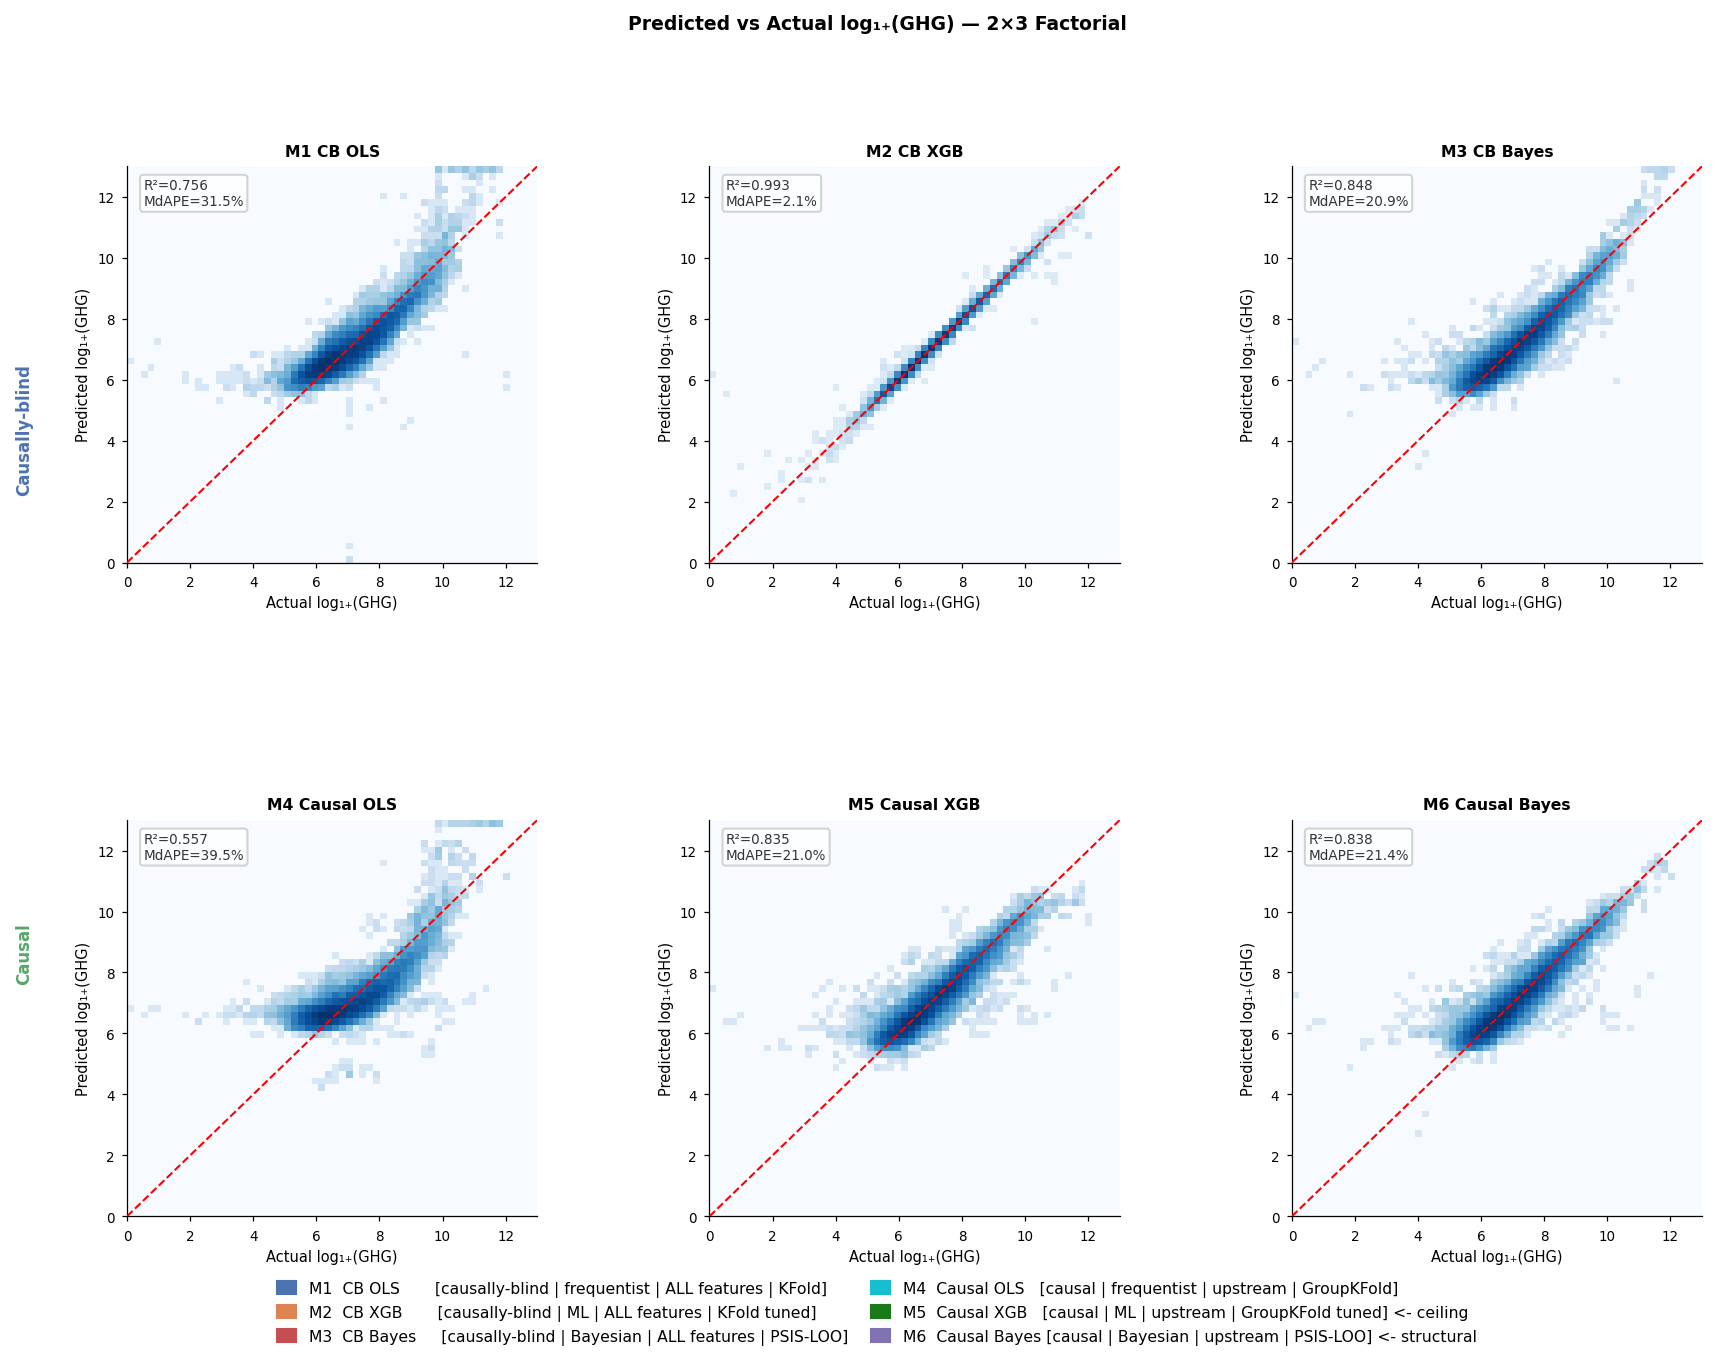
\includegraphics[width=0.95\linewidth]{figures/fig_pred_vs_actual.png}
\caption*{\textbf{Figure 5.4. Predicted vs actual $\log_{1+}$(GHG) for all six models, 2$\times$3 factorial.} M2's near-perfect diagonal collapse ($R^2 = 0.993$) is the accounting artefact made visible; the pattern is absent from every other model. M5 and M6 produce scatter-equivalent plots, confirming that functional form does not matter once the target quantity is fixed by the tested DGP. Author's analysis of Chicago Energy Benchmarking data.}
\end{figure}

\textbf{M2: accounting artefact mechanism.} SHAP group attribution (Figure 5.5a) quantifies what drives M2's metrics: energy mediators account for 57.2\% of M2's total predictive signal; derived/circular features (GHG intensity, site and source EUI, Energy Star score, Chicago Energy Rating) contribute a further 15.0\%; together 72.2\% of M2's signal comes from features that are either post-treatment or tautological. The dominant individual contributor is \code{electricity\_use\_kbtu} (42.3\%), through which XGBoost learns the direct EPA emission-factor mapping rather than any upstream causal structure. Only 26.1\% of M2's signal derives from upstream causal features, the only feature set causally valid at deployment and the sole basis on which M5 operates. Figures 5.5b and 5.5c make the mechanism concrete: even the highest-ranking upstream causal feature (log floor area, mean |SHAP| $\approx$0.23) is outweighed more than two-to-one by electricity alone, and the beeswarm confirms that the learned relationship is monotone and tight, the signature of a direct emission-factor mapping rather than a causal model of building characteristics.

\begin{figure}[tbp]
\centering
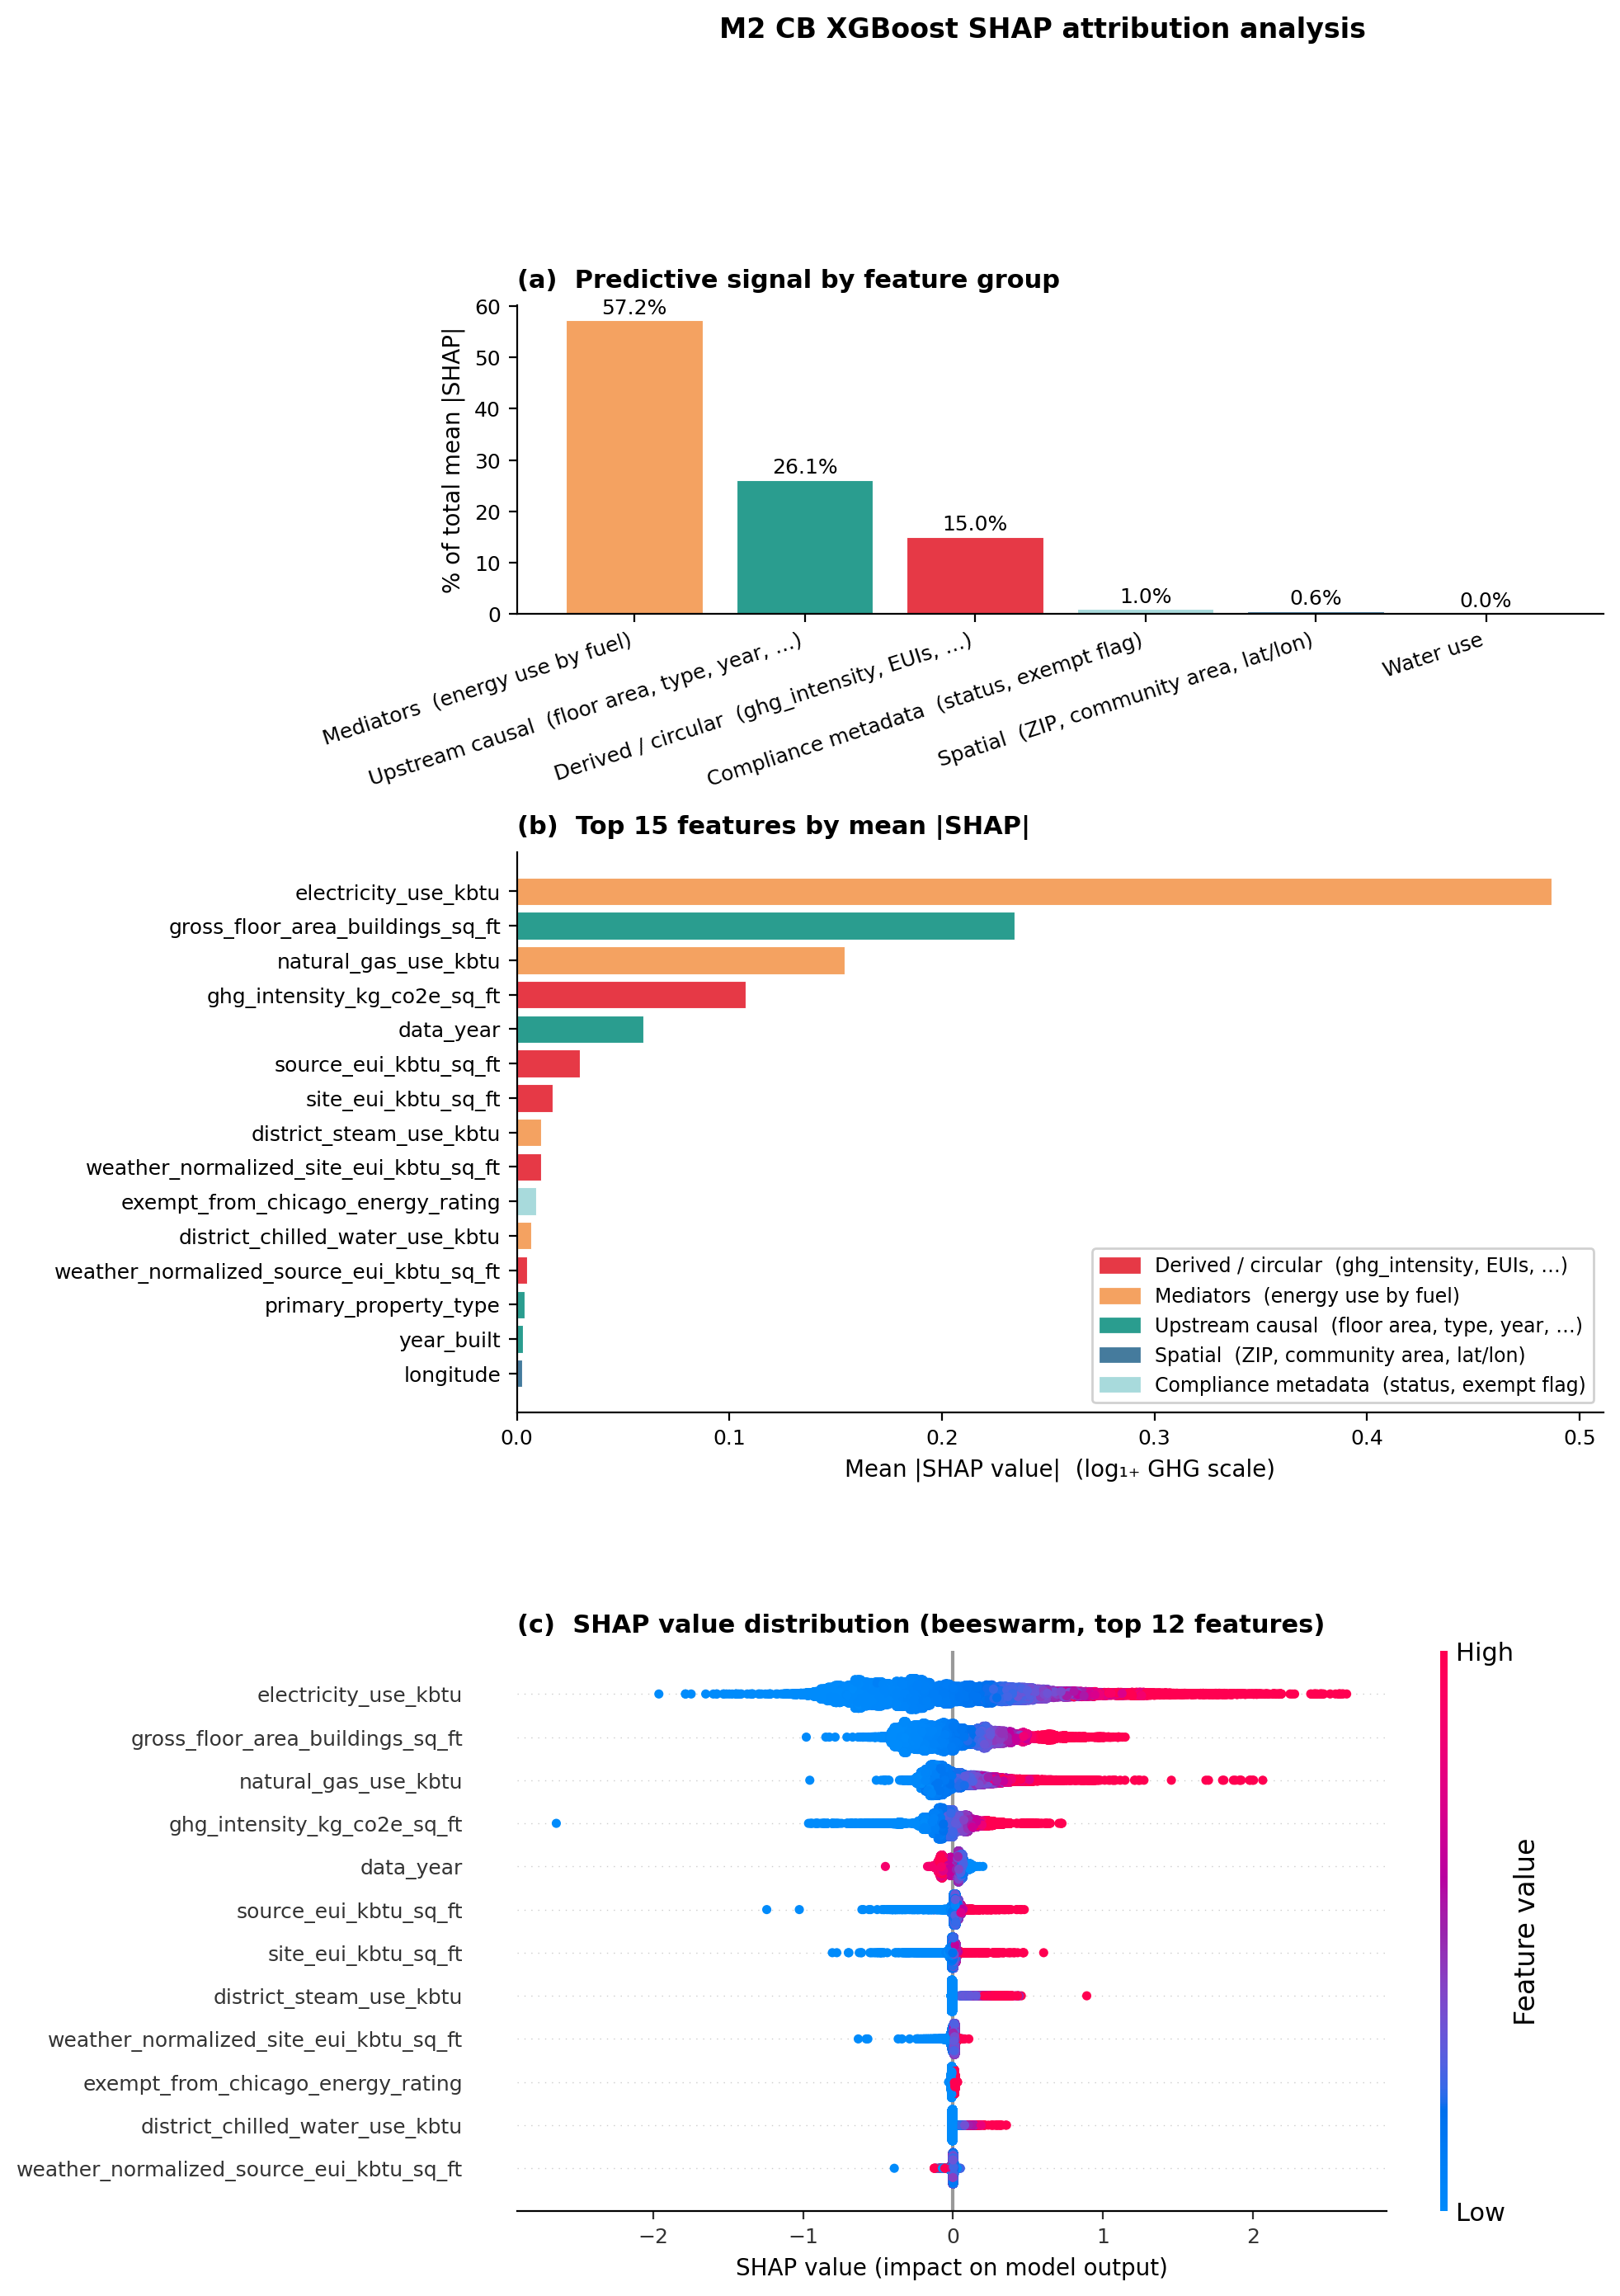
\includegraphics[width=0.8\linewidth]{figures/fig_shap_combined.png}
\caption*{\textbf{Figure 5.5. M2 CB XGBoost SHAP attribution analysis.} (a) Predictive signal by feature group: energy mediators account for 57.2\%; derived/circular features (GHG intensity, EUI variants, Energy Star score) contribute a further 15.0\%; together 72.2\% comes from features unavailable or causally invalid at deployment; upstream causal features contribute 26.1\%. (b) Top 15 features by mean |SHAP|: \code{electricity\_use\_kbtu} dominates at mean |SHAP| $\approx$0.49, more than double the next feature (\code{gross\_floor\_area\_buildings\_sq\_ft} at $\approx$0.23); apart from floor area, the top positions are held by mediators (orange) and derived/circular features (red), with the remaining upstream causal features (teal) in the lower half. (c) SHAP value distribution (beeswarm, top 12 features): \code{electricity\_use\_kbtu} and \code{natural\_gas\_use\_kbtu} show a strong monotone positive relationship, confirming XGBoost has learned the EPA emission-factor mapping directly; upstream causal features produce narrow, low-magnitude bands. Author's analysis of Chicago Energy Benchmarking data.}
\end{figure}

\textbf{M3 vs M6: the Bayesian gap.} The near-zero gap between M3 (20.9\%) and M6 (21.4\%) reflects a structural mis-match between M3's likelihood and the true EPA formula. The EPA GHG formula is additive in the original scale (GHG $= \sum_f \text{fuel}_f \times \varepsilon_f$); M3 models $\log_{1+}(\text{GHG})$ as linear in standardised fuel use, a specification that cannot represent an additive-in-levels sum: in log space, $\log\bigl(\sum_f \text{fuel}_f \times \varepsilon_f\bigr)$ is nonlinear in the individual fuels, so the log-linear coefficients cannot recover the emission-factor magnitudes. The posterior mediator slopes confirm the mis-match (Figure 5.6a): electricity use, the dominant driver of M2's 42.3\% SHAP signal, receives a posterior mean of only $+0.078$ on the standardised log scale, compared to log floor area at $+0.898$. District steam and all other fuel have 89\% posterior intervals that span zero. The log-linear specification assigns most explanatory power to log floor area (a proxy for scale that remains monotone with GHG even after log-transformation) and extracts only marginal signal from the mediators. M3 therefore cannot exploit its mediator access, and the 0.4 pp gap to M6 reflects near-equivalent predictive information rather than a genuine trade-off between mediator access and IPW correction. Figure 5.6b shows that M6's floor-area slope ($+0.979$) exceeds M3's ($+0.898$): without mediator slopes to distribute the scale signal, M6 assigns more explanatory weight to floor area.

\begin{figure}[tbp]
\centering
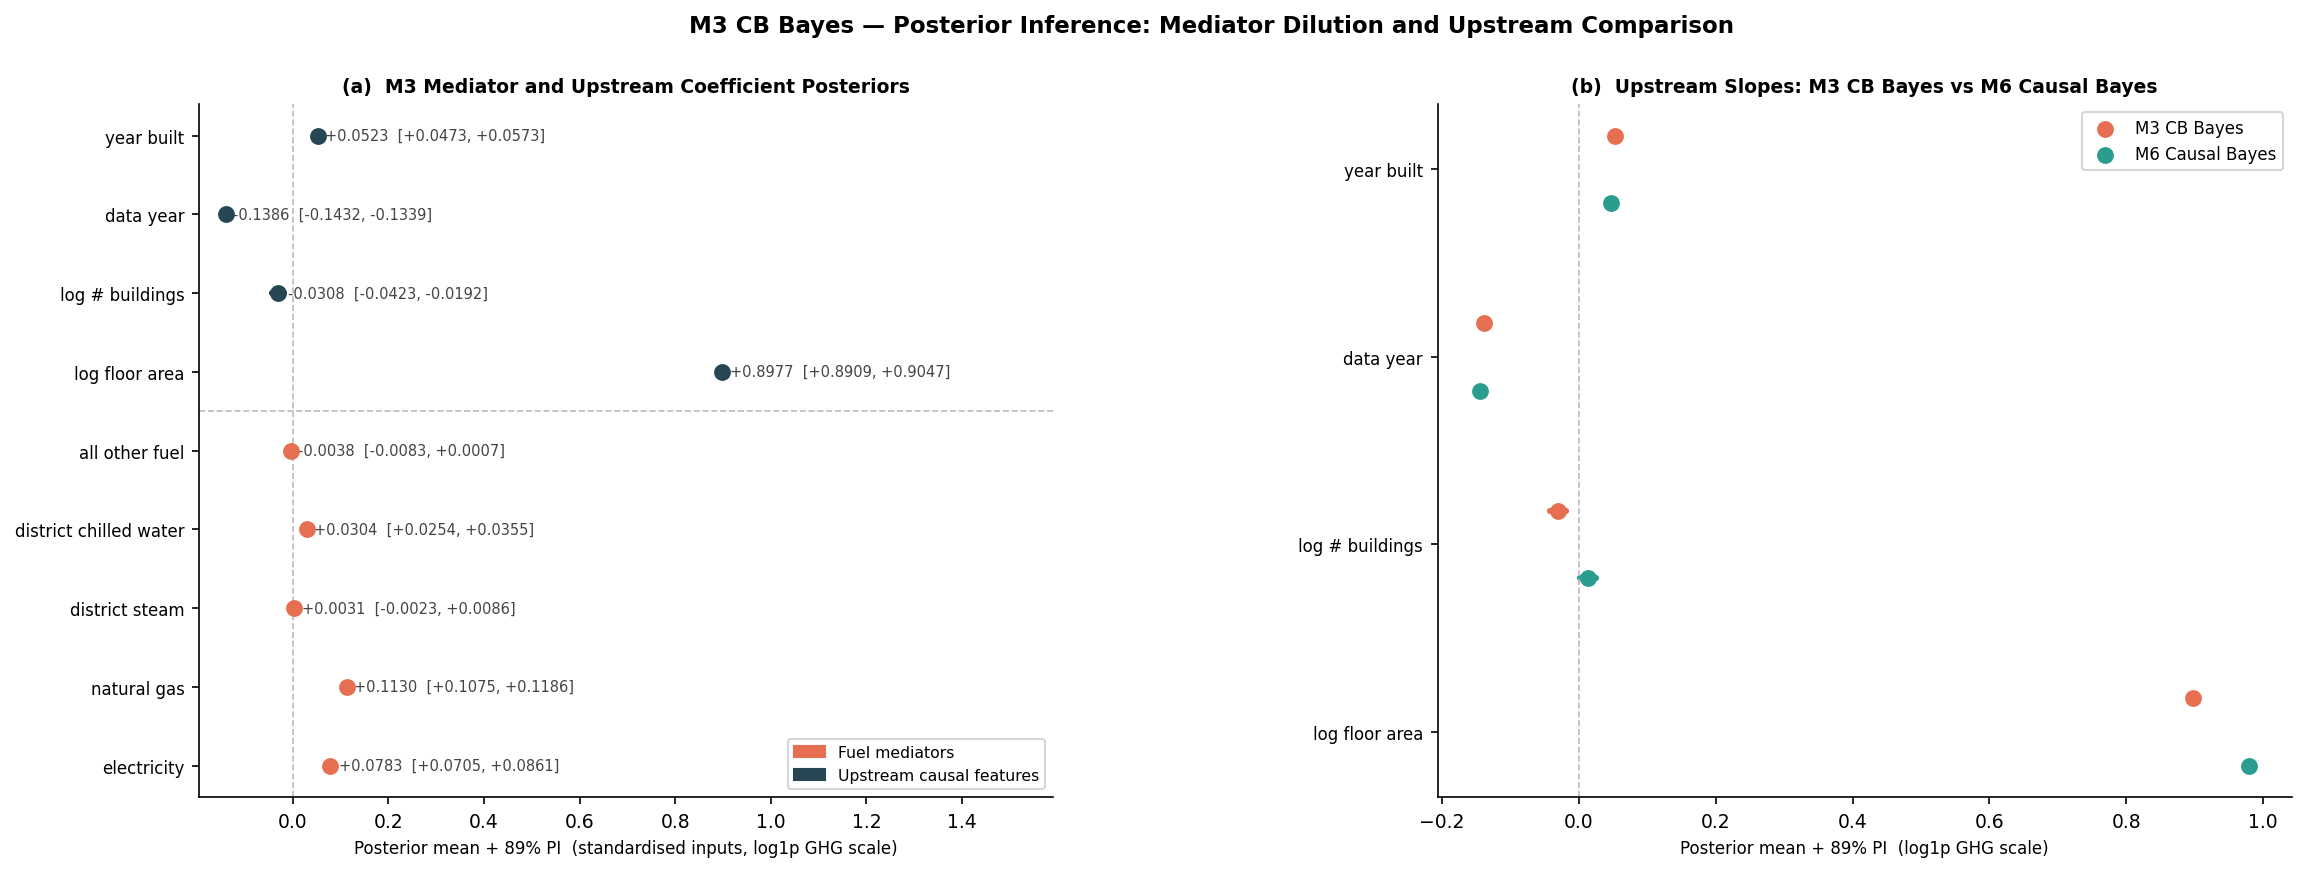
\includegraphics[width=0.95\linewidth]{figures/fig_m3_combined.png}
\caption*{\textbf{Figure 5.6. M3 CB Bayes posterior inference.} (a) Mediator and upstream coefficient posteriors (89\% PI): fuel mediator slopes (orange) are small relative to log floor area (teal, $+0.898$); electricity and natural gas are positive and precisely estimated but far below the floor-area coefficient; district steam and all other fuel have intervals spanning zero; the log-linear likelihood cannot recover the EPA emission-factor structure, leaving floor area to absorb the bulk of the explanatory signal. (b) Upstream slope comparison, M3 CB Bayes vs M6 Causal Bayes: M6's log floor-area slope ($+0.979$) exceeds M3's ($+0.898$) because M6 has no mediator slopes to share the scale signal with; the remaining upstream slopes are directionally consistent across models. Author's analysis of Chicago Energy Benchmarking data.}
\end{figure}

\textbf{Causally-blind deployment behaviour.} M2's deployment median (641 metric tons) is not near-zero: non-compliant buildings receive training-median imputation for all derived fields, so M2 predicts approximately $\hat{y}_i \approx \bar{g} \cdot a_i$ where $\bar{g}$ is the median GHG intensity and $a_i$ is floor area, the only feature that still varies across buildings. The prediction is numerically plausible but causally invalid; a practitioner without causal domain knowledge might accept it.

\subsubsection*{Discussion of Experimental Results}

Three limits bound these results. First, IPW corrects for selection on observed upstream characteristics; the unobserved component of selection (management practices, voluntary retrofits, tenant behaviour) remains uncorrected. The maximum normalised weight of 1.32 indicates moderate observed distortion, but the unobserved component is unbounded. The smallness of that maximum weight also bounds how much the correction does on this dataset: with weights this close to one, IPW shifts the causal estimates only modestly, so Chicago is a mild test of the selection machinery rather than a stringent one. The convergence and deployment results are therefore demonstrated under weak observed selection; a programme with a sharper gate or thinner overlap would exercise the correction far harder, and whether the same agreement survives there is exactly the cross-class replication Section 8 calls for. Second, the deployment test establishes ordinal plausibility relative to the compliant-building distribution; it does not provide ground-truth GHG for the 5,510 non-compliant building-year records, none of which have observed energy data. Third, M3's near-identical deployment prediction (1,025 metric tons versus M6's 1,043 metric tons) does not imply causal equivalence: M3's mediator slopes are too small to shift predictions materially from what upstream features alone produce, so the agreement reflects diluted coefficients rather than inherent Bayesian robustness to the compliance gate.

The 0.4 percentage-point gap between M5 and M6 means that functional form is not a source of uncertainty once the DGP is fixed: a flexible non-parametric estimator and a structural Bayesian model arrive at the same prediction when trained on the same causal foundation. That agreement is what the tested DGP predicted (Section 5.5), and within the limits stated above it corroborates the structure; it does not certify the structure beyond the observed support, where no ground truth exists. Subject to those limits, the posterior parameters of M6 are interpretable as estimates of causal quantities, and Section 6 examines them.

